\documentclass[bibtotocnumbered]{article}
\usepackage[english]{babel}

\usepackage[utf8]{inputenc}
\usepackage{amsmath}
\usepackage{titlesec}
\usepackage{xcolor}
\usepackage{sectsty}
\usepackage[T1]{fontenc}
\usepackage{XCharter}
\usepackage{glossaries}
\usepackage{graphicx}
\usepackage[toc,page]{appendix}
\usepackage[
top    = 1in,
bottom =1in,
left   = 1in,
right  = 1in]{geometry}
\usepackage[parfill]{parskip}
\usepackage[utf8]{inputenc}
\usepackage{fancyhdr}
\usepackage[backend=biber, style=authoryear]{biblatex}
\addbibresource{refs.bib}
\usepackage{hyperref}
\setcounter{secnumdepth}{4}

\titleformat{\paragraph}
{\normalfont\normalsize\bfseries}{\theparagraph}{1em}{}
\titlespacing*{\paragraph}
{0pt}{3.25ex plus 1ex minus .2ex}{1.5ex plus .2ex}
\begin{document}
\section{Designs}
\section{UI Design}
The User interface for this project is designed with the average musician in mind, and the interfaces that user would normally have used. With this in mind, the designs explained below and shown in Appendix D are inspired by other music applications in common usage.

\subsubsection{Explanation of how the current designs link together}
The first image in Appendix D shows the main display when a collection is opened - to the left, an import button, which allows the user to import a new piece into the collection and opens a popup window shown in image 4, and a refresh button. The refresh button forces the system to recheck the folder for new pieces the user may have copied using their operating system's file browser.

Below these two buttons, a search bar is displayed. In the fourth image, the box marked "on text entry in search boxes" shows how search data is displayed, and the label "to render window on click" indicates that when a piece is clicked, the main pane will update to show something similar to the second image in the appendix.

Below the search box optional panes are open by default. The first is the collection browser, which organises all pieces by the option selected in the drop down. 

Following this, the playlist browser, which shows all playlists the user has created. The add symbol at the bottom opens up a pop up window, shown in image 4. The piece search box used in this will be the same as in the main window, and the user may delete pieces by selecting them in the Piece List and pressing the delete button on their keyboard, or right clicking.

Below the playlist browser, a similar window shows playlists the system has generated based on the metadata database. These are not deletable and will automatically add new pieces to the appropriate list whenever the collection is refreshed.

To the right of the three panes, the main window is used for displaying playlists or sheet music. The sheet music view is displayed in image 2, along with two further optional panes displayed to the right of this pane. The first shows the metadata the system has extracted - where there are other pieces with the same options, the value of each metadata item is clickable, for example, the word "Bartok" in the image. 

Below this pane, if the user has selected this piece from the collection browser, a pane displaying the playlists this piece belongs to will display.  Beneath the list, a search box shows, allowing the user to add the piece to a pre existing playlist.

If the user has selected this piece from the playlist view, shown in image 3, the list of other pieces in this playlist will show in the second pane to the right of the main window.

Above the main pane in image two shows some buttons useful to the user. The two popups below and to the right of this graphic show the window which displays when "play selected parts " is clicked, and the window which displays when draw is clicked. Both of these will display as panes beneath the sheet music, which will close when the user clicks the "x" button in the top left corner.

The third image of the appendix shows the updated main pane when a playlist is selected from either of the playlist listings. The title is editable in place using the pen shaped icon, and the column titles displayed are also editable from this page.
\subsubsection{Musician feedback survey}
The survey in Appendix E shows an example form which will be given to a musician, who will feedback on how easy the UI is to use and any updates which should be made to improve it. This feedback session will be performed after the initial sketches are made into an application, which will be created, evaluated and then linked to the main system once the developer and participants are happy with the design.
\begin{appendices}
\section{Revised computerised class diagram}
\section{Initial User Interface Design}
\subsection{Main Display}
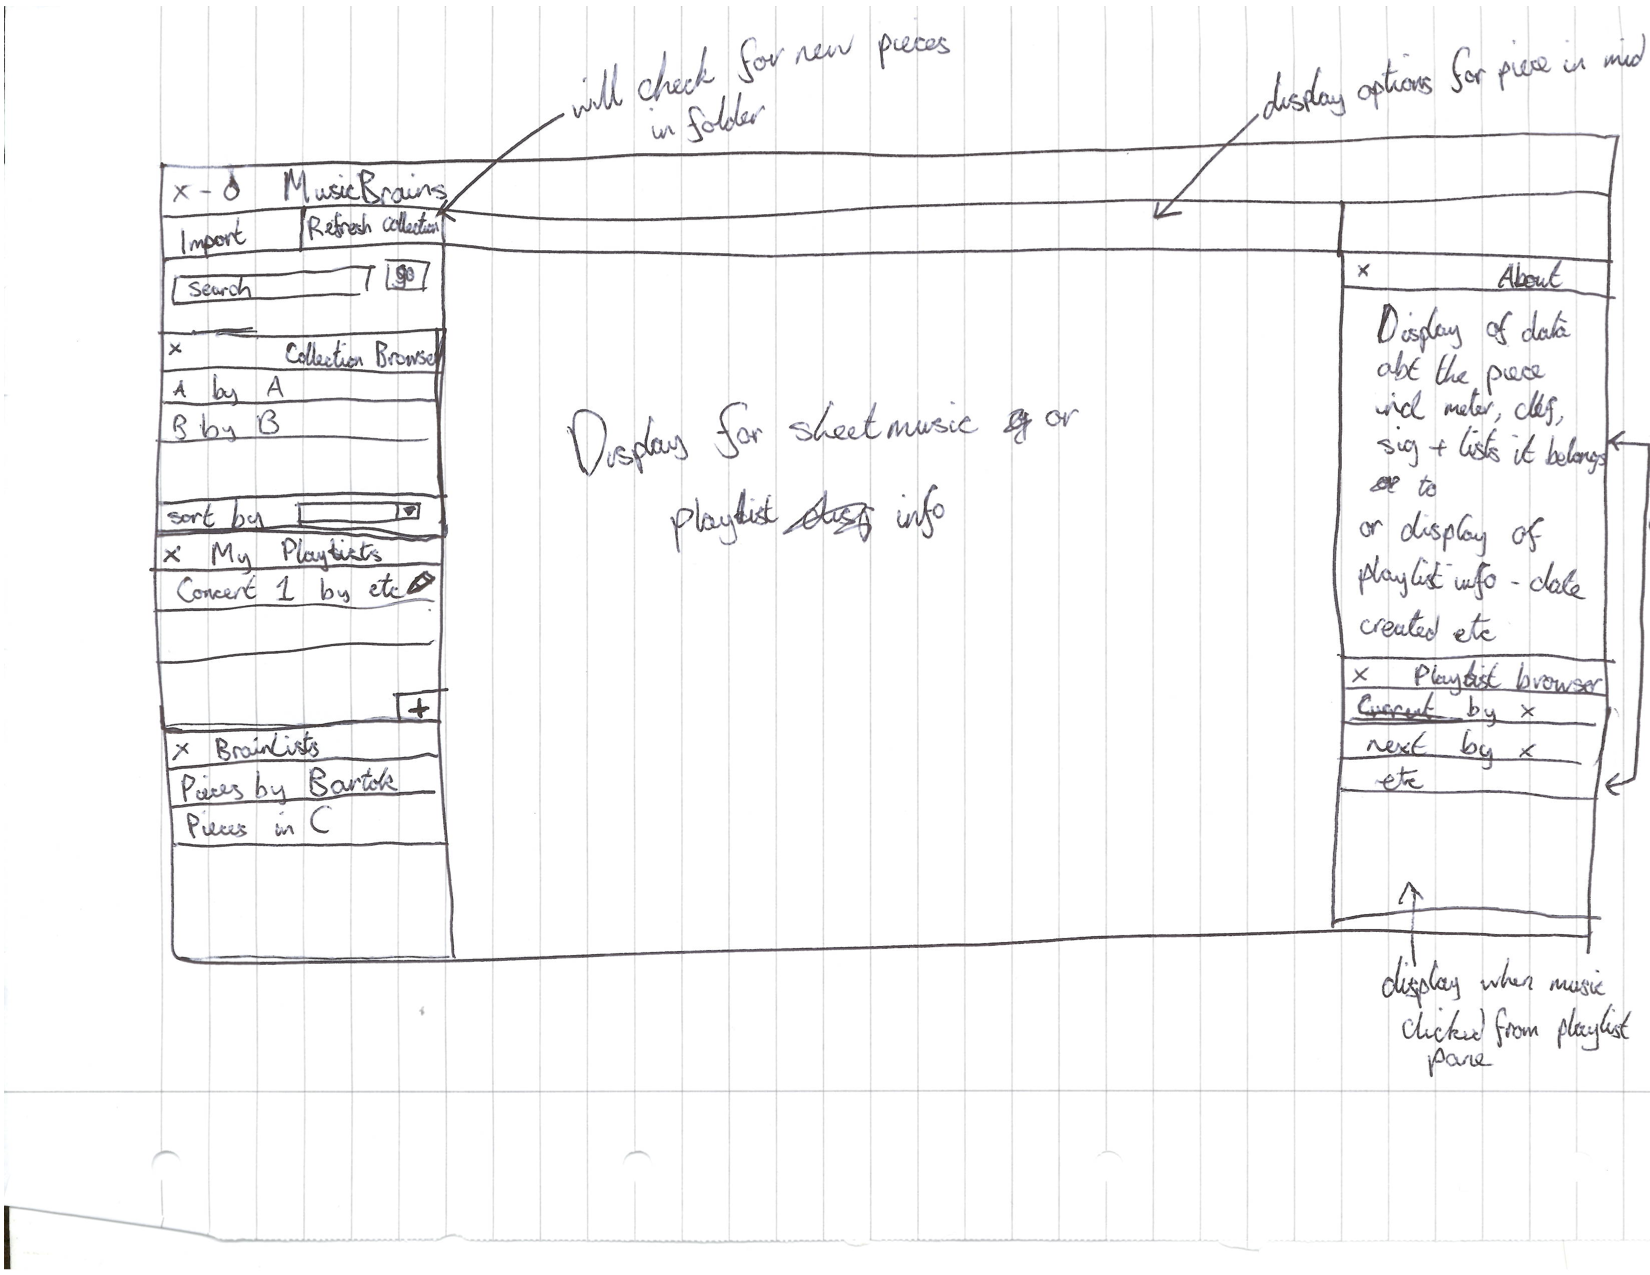
\includegraphics[width=500pt]{main_view.png}
\subsection{Changes to main display when sheet music selected}
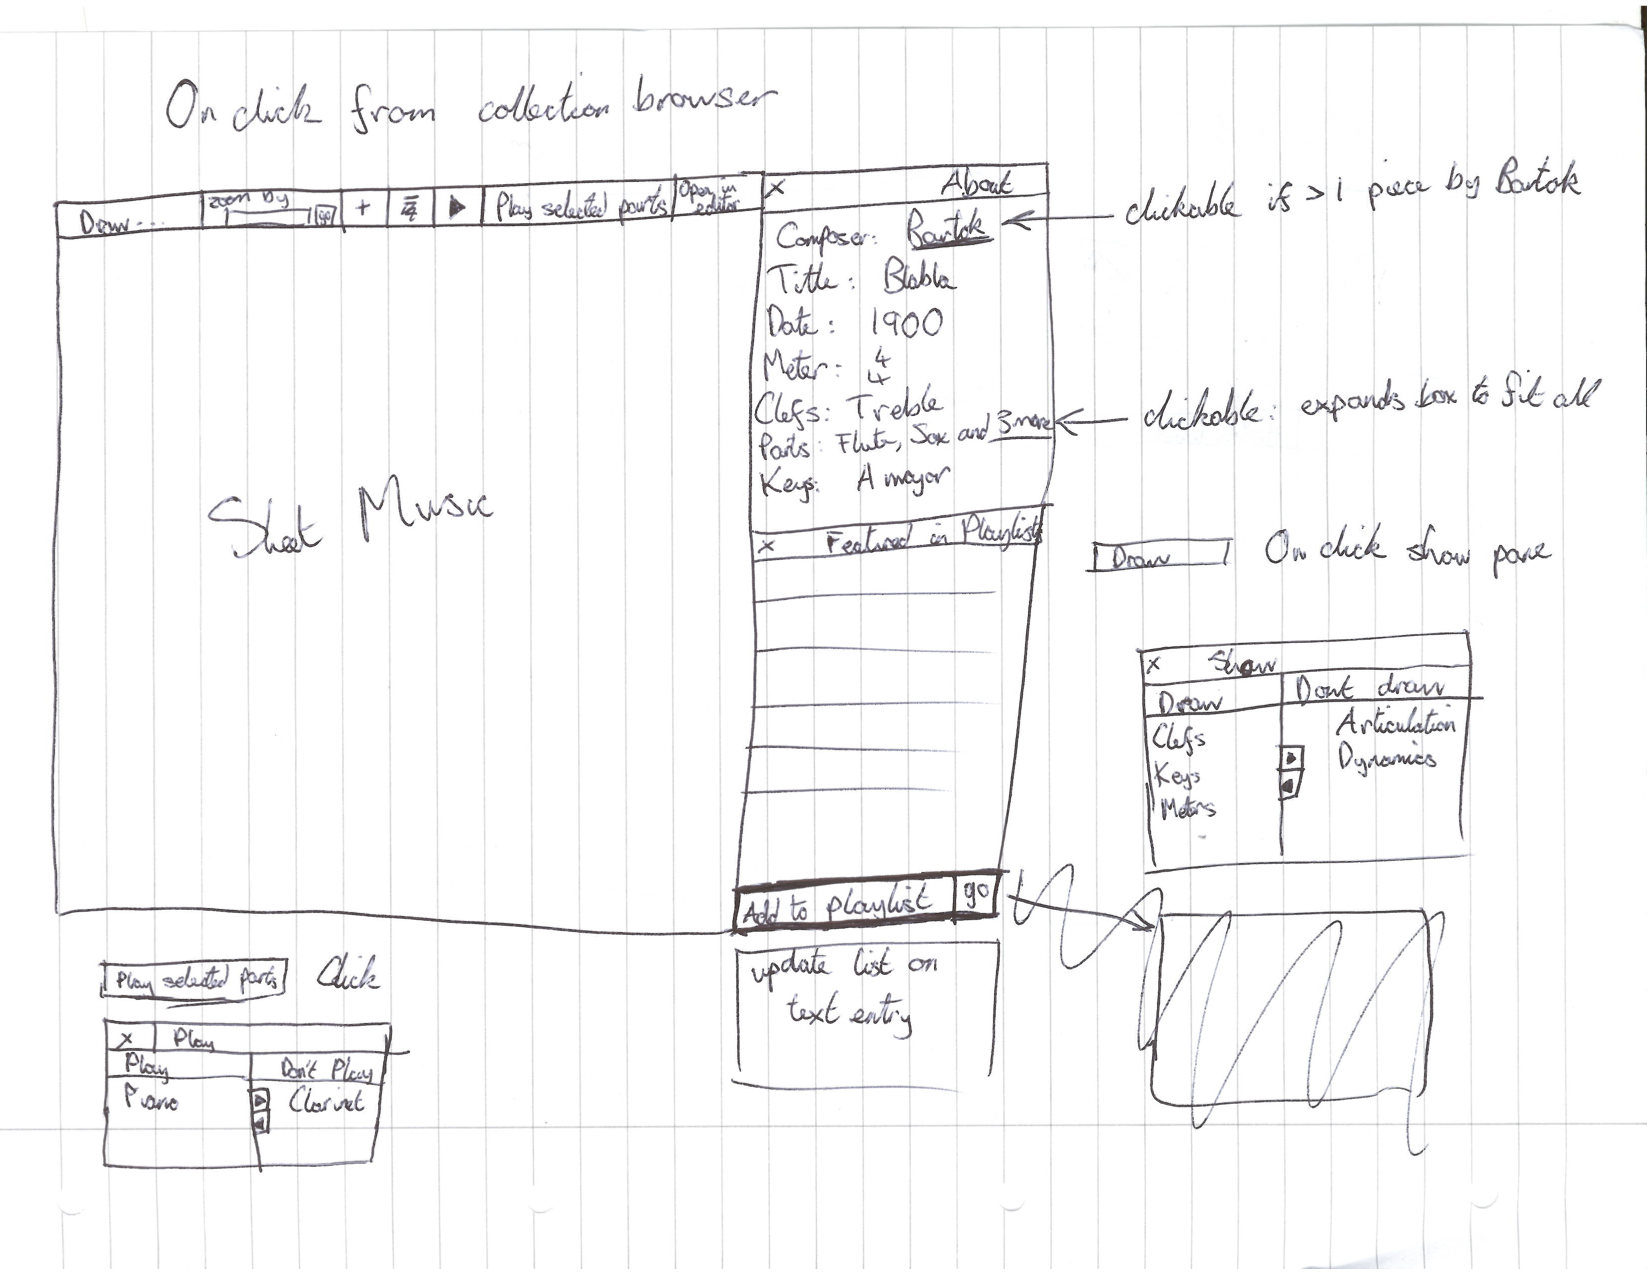
\includegraphics[width=400pt]{sheet_music_view.png}
\subsection{Changes to main display when playlist is selected}
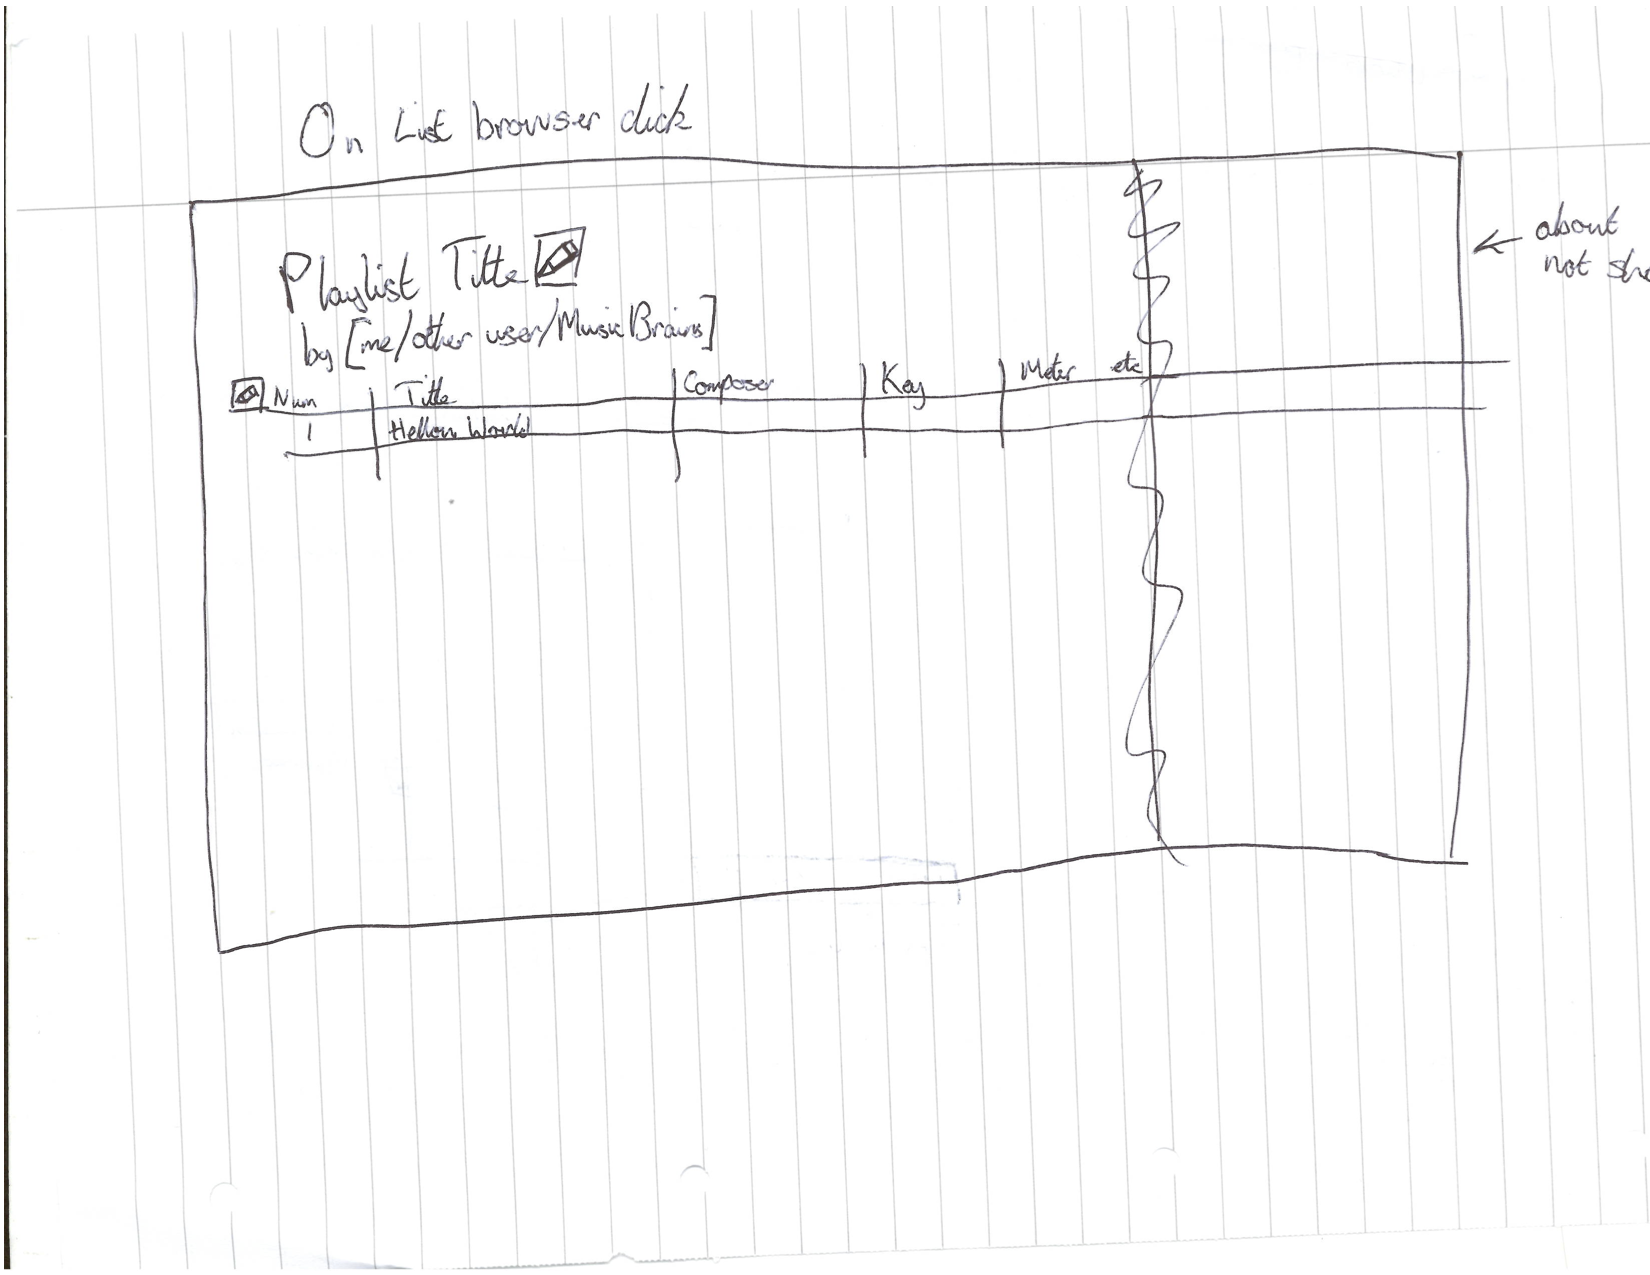
\includegraphics[width=500pt]{playlist_view.png}
\subsection{Other Panes and Popup windows}
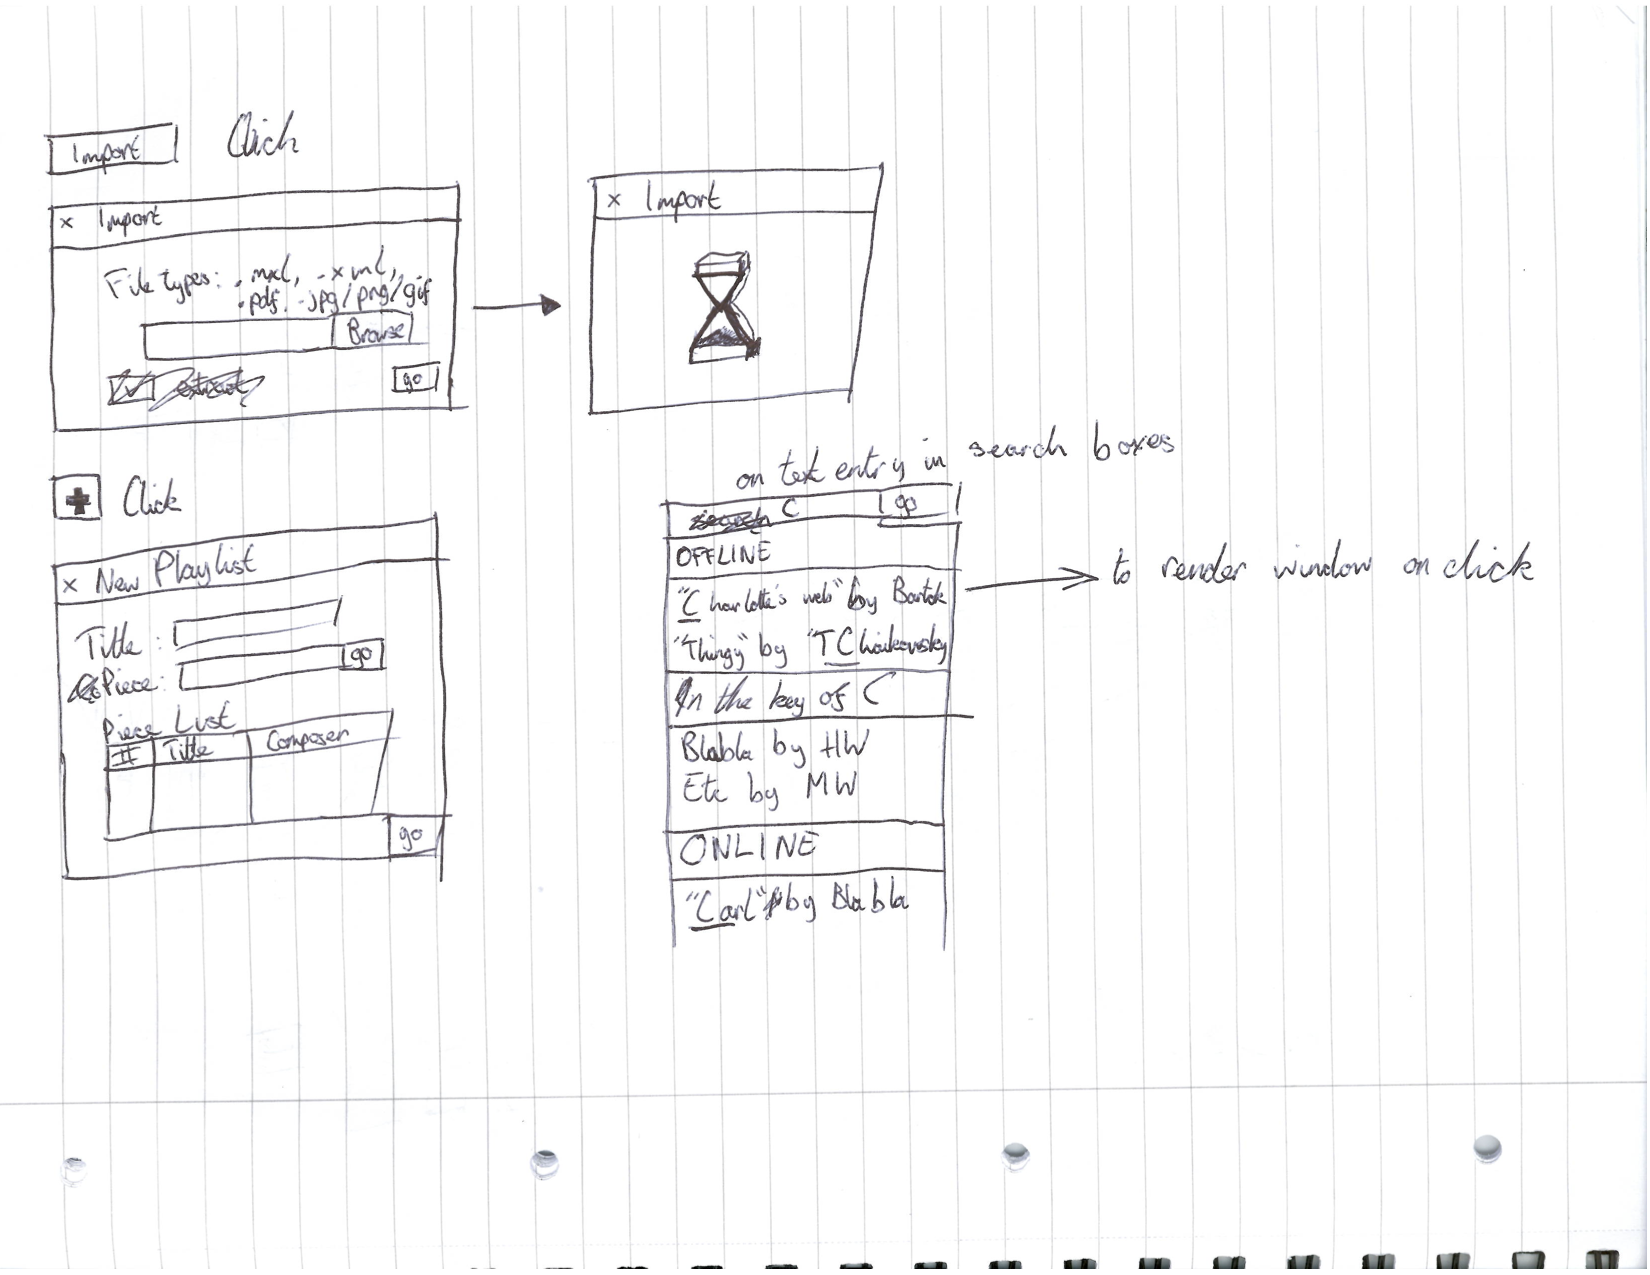
\includegraphics[width=500pt]{other_panes_and_popups}
\end{appendices}

\end{document}
